\sectioncounter{19}

\section{三角函数的图象和性质}

\subsection{知识梳理}
根据三角函数线可以分别列出正弦函数 $y=\sin x$, 余弦函数 $y=\cos x$ 
和正切函数 $y=\tan x$ 的函数值表, 并作出它们在一个周期内的图象, 如图 \ref{fig-190223-2200} 和图 \ref{fig-190223-2205} 所示.
\begin{figure}[htb]
\small
\centering
\begin{minipage}[c]{0.45\linewidth}
    \centering
    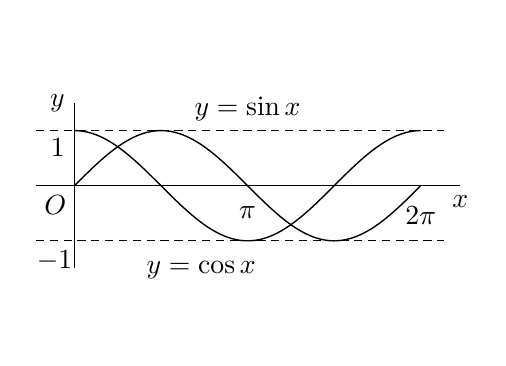
\begin{tikzpicture}[scale=0.7]
      \draw[\myaxisarrow] (-0.7,0) -- (7,0) node[below] {$x$};
      \draw[\myaxisarrow] (0,-1.5) -- (0,1.5) node[left] {$y$};
      \draw[line width=0.5pt,smooth,samples=100,domain=0:6.28] 
        plot(\x,{sin(\x*180/pi)});
      \draw[line width=0.5pt,smooth,samples=100,domain=0:6.28] 
        plot(\x,{cos(\x*180/pi)});
      
      \draw[densely dashed] (-0.7,1)--(6.7,1) (-0.7,-1)--(6.7,-1);
      \draw (0,1) node[anchor=45] {$1$} (0,-1) node[anchor=45] {$-1$};
      \draw (0,0) node[anchor=45] {$O$};
      \draw (2*pi,-0.2) node[below] {$2\pi$};
      \draw (pi,-0.2) node[below] {$\pi$};
      \draw (pi,1) node[above] {$y=\sin x$};
      \draw (2.3,-1.2) node[below] {$y=\cos x$};
      \draw (0,-2.6) node {} (0,2.7) node {};
    \end{tikzpicture}
\caption{}\label{fig-190223-2200}
\end{minipage}
\hskip 0.5cm%
\begin{minipage}[c]{0.45\linewidth}
    \centering
    \begin{tikzpicture}[scale=0.7]
      \draw[\myaxisarrow] (-2.5,0) -- (2.5,0) node[below] {$x$};
      \draw[\myaxisarrow] (0,-2.6) -- (0,2.5) node[left] {$y$};
      \draw[line width=0.5pt,smooth,samples=100,domain=-1.2:1.2] 
        plot(\x,{tan(\x*180/pi)});
      \draw[line width=0.4pt,densely dashed] 
        (-1.57,-2.4) -- (-1.57,2.3);
      \draw[line width=0.4pt,densely dashed] 
        (1.57,-2.4) -- (1.57,2);
      
      \draw (0.4,-0.4) node {$O$};
      \draw (-1.5,-0.7) node[left] {$-\dfrac{\pi}2$};
      \draw (0.9,-0.7) node[right] {$\dfrac{\pi}2$};
      \draw (1.25,2.5) node[right] {$y=\tan x$};
      \draw (-3,0) node {};
    \end{tikzpicture}
\caption{}\label{fig-190223-2205}
\end{minipage}
\end{figure}

由三个函数图象可以列出以下性质表 (结合图象记忆, 表中 $k\in\mathbb{Z}$):
{\extrarowheight=7pt\small
\begin{center}
    \begin{tabular}{cccccc}
        & 定义域 & 值域 & 最小正周期 & 对称中心 & 对称轴 \\
       \hline
      $y=\sin x$ & $\mathbb{R}$ & $[-1,1]$ & $2\pi$ & 
        $(k\pi,0)$ & $x=\dfrac{\pi}2+k\pi$\\
      $y=\cos x$ & $\mathbb{R}$ & $[-1,1]$ & $2\pi$ & 
        $\Big(\dfrac{\pi}2+k\pi,0\Big)$ & $x=k\pi$ \\
      $y=\tan x$ & $\Big\{x\neq\dfrac{\pi}2+k\pi\Big\}$ & $\mathbb{R}$ &
        $\dfrac{\pi}2$ & $\Big(\dfrac{k\pi}2,0\Big)$ & 无
    \end{tabular}
\end{center}
\begin{center}
    \begin{tabular}{ccc}
           & 奇偶性 & 单调性 \\
       \hline
      $y=\sin x$ & 奇 &
        $\Bigl[-\dfrac{\pi}2+2k\pi,\dfrac{\pi}2+2k\pi\Bigr]\nearrow$,
        $\Bigl[\dfrac{\pi}2+2k\pi,\dfrac{3\pi}2+2k\pi\Bigr]\searrow$   \\
      $y=\cos x$ & 偶 & 
        $\Bigl[-\pi+2k\pi,2k\pi\Bigr]\nearrow$, 
        $\Bigl[2k\pi,\pi+2k\pi\Bigr]\searrow$                \\
      $y=\tan x$ & 奇 & 
        $\Bigl(-\dfrac{\pi}2+k\pi,\dfrac{\pi}2+k\pi\Bigr)\nearrow$
    \end{tabular}
\end{center}}

由函数图象变换可知 $y= A\sin(\omega x+ \varphi)$ $(\omega\neq 0)$ 的最小正周期 $T= \dfrac{2\pi}{|\omega|}$, 对称轴对应最值点且对称中心对应零点, 而 $y= |\sin x|$ 的最小正周期是 $\pi$. 同样可知 可知 $y= A\cos(\omega x+ \varphi)$ $(\omega\neq 0)$ 的最小正周期 $T= \dfrac{2\pi}{|\omega|}$.

\lianxi
\begin{exercise}
    求函数 $y=\tan\Big(2x-\dfrac\pi3\Big)$ 的定义域.
\end{exercise}
\beginsolution
    由题意, $2x-\dfrac\pi3\neq \dfrac\pi2+k\pi$, 则所求定义域为
    \[\biggl\{x\biggm| x\neq \frac{5\pi}{12}+ \frac{k\pi}{2},\ 
        k\in\mathbb{Z}\biggr\}.\]
\endsolution

\begin{exercise}
    求函数 $y=\sin x$ $\Big(\dfrac\pi6\leqslant x\leqslant 
      \dfrac{2\pi}3\Big)$ 的值域.
\end{exercise}
\beginsolution
    由正弦线知, $y\in\biggl[\dfrac12,1\biggr]$.
\endsolution

\begin{exercise}
    求函数 $y=\sin\Big(2x+\dfrac\pi4\Big)$ 单调递增区间.
\end{exercise}
\beginsolution
    由正弦函数图象知, 单调递增区间满足
    \[2x+\dfrac\pi4\in \biggl[-\frac\pi2+2k\pi,\frac\pi2+2k\pi\biggr],\quad 
    k\in\mathbb{Z},\]
    则所求单调递增区间为 $\biggl[-\dfrac{3\pi}8+k\pi,\dfrac{\pi}8++k\pi\biggr]$, $k\in\mathbb{Z}$.
\endsolution

\begin{exercise}
    已知函数 $f(x)=ax^2 \sin x+b\tan x$, $f\Bigl(-\dfrac\pi4\Bigr)=3$, 求 $f\Big(\dfrac\pi4\Big)$ 的值.
\end{exercise}
\beginsolution
    可验证 $f(-x)= -f(x)$, 即 $f(x)$ 为奇函数, 所以 
    \[f\Big(\dfrac\pi4\Big)= -f\Bigl(-\dfrac\pi4\Bigr)= -3.\]

    \varexercise 若函数 $f(x)=ax^2 \sin x+b\tan x+ 2$, $f\Bigl(-\dfrac\pi4\Bigr)=3$, 则 $f(x)-2$ 为奇函数, 所以
    \[\begin{gathered}
        f\Bigl(-\dfrac\pi4\Bigr)- 2
        = -\biggl[f\Big(\dfrac\pi4\Big)- 2\biggr],\\
        f\Bigl(-\dfrac\pi4\Bigr)+f\Big(\dfrac\pi4\Big)=4,\quad
            \text{即}\quad f\Big(\dfrac\pi4\Big)= 1.
    \end{gathered}\]
\endsolution

\begin{exercise}
    函数 $y=\sin 2x$ 的图象向右平移 $\varphi$ ($\varphi>0$) 个单位长度, 
    得到的图象关于直线 $x= \dfrac\pi6$ 对称, 求 $\varphi$ 的最小值.
\end{exercise}
\beginsolution
    方法一: 平移后图象的解析式为 $y=\sin 2(x-\varphi)$, 且将 $x= \dfrac\pi6$ 代入得 $\sin\biggl(\dfrac\pi3- 2\varphi\biggr)= \pm1$, 则
    \[\frac{\pi}{3}- 2\varphi= \frac{\pi}{2}+k\pi,\quad k\in\mathbb{Z},\]
    所以 $\varphi= -\dfrac{\pi}{12}+ \frac{k\pi}2$, $k\in\mathbb{Z}$. 由 $\varphi>0$ 知, 当 $k=1$ 时, $\varphi= \dfrac{5\pi}{12}$ 最小.

    方法二: 作出 $y=\sin 2x$ 的图象, 
    \mymarginpar{\begin{center}
        \includegraphics[align=u,scale=1.5]{2021-0227-1100-crop}
    \end{center}}
    直接观察对称轴可知, 至少应平移 $\dfrac\pi4+ \dfrac\pi6= \dfrac{5\pi}{12}$ 才合题意.
\endsolution

\subsection{要点导学\quad 各个击破}
\subsubsection{三角函数相关的定义域和值域问题}
\begin{example}
    求函数的定义域:
    
    (1) $f(x)=\lg(\sin x-\cos x)$;\quad
    (2) $g(x)=\dfrac{\sqrt{2\cos x+1}}{\tan x}$.
\end{example}
\beginsolution
    (1) 只需 $\sin x-\cos x>0$ 即 $\sin x>\cos x$, 再由正弦线和余弦线可知,
    \[x\in\biggl(\frac\pi4+2k\pi, \frac{5\pi}4+2k\pi\biggr),\quad
        k\in\mathbb{Z}.\]

    (2) 由题意, $2\cos x+1\geqslant 0$ 且 $\tan x\neq 0$. 前者表明 $\cos x\geqslant -\dfrac12$, 即
    \[x\in \biggl[-\frac{2\pi}{3}+ 2k\pi, \frac{2\pi}{3}+ 2k\pi\biggr],\quad k\in\mathbb{Z},\]
    后者表明 $x\neq \dfrac{k\pi}2$, $k\in\mathbb{Z}$, 取交集即可.
\endsolution

\begin{example}
    求函数的值域:
    
    (1) $f(x)=\sin x$, $x\in[-135^\circ,45^\circ]$;\quad
    (2) $g(x)=\cos x$, $x\in\Bigl(-\dfrac{\pi}4,\dfrac{3\pi}4\Bigr)$.
\end{example}
\beginsolution
    由正弦线和余弦线知, $f(x)\in\biggl[-1, \dfrac{\sqrt2}2\biggr]$, $g(x)\in\biggl(\dfrac{\sqrt2}2, 1\biggr]$.
\endsolution

\lianxi
\begin{exercise}[s]
    求函数 $y= \sqrt{2+\log_{\frac12} x}+ \sqrt{\tan x}$ 的定义域.
\end{exercise}
\beginsolution
    由题意, $2+\log_{\frac12} x\geqslant 0$ 且 $\tan x\geqslant 0$. 前者表明 $\log_{\frac12} x\geqslant -2$, 即 $0<x\leqslant 4$, 
    \mymarginpar{此处由对数的定义, $x>0$.}
    结合后者知,
    \[x\in\biggl(0,\frac\pi2\biggr)\cup (\pi,4].\]
\endsolution

\subsubsection{三角函数的单调性和对称性问题}
\begin{example}
    已知函数 $f(x)=-1+2\sqrt3 \sin x\cos x+2\cos^2 x$.
    
    (1) 求 $f(x)$ 的单调递减区间;
    
    (2) 求 $f(x)$ 图象上离原点最近的对称中心的坐标.
\end{example}
\beginsolution
    先化简 $f(x)$ 的解析式,
    \[f(x)= \sqrt3\sin2x+ \cos2x
        = 2\sin\biggl(2x+\frac\pi6\biggr).\]
    
    (1) 对 $f(x)$ 的单调递减区间,
    \[\begin{gathered}
        2x+\frac\pi6\in \biggl[-\frac\pi2+2k\pi, 
            \frac\pi2+2k\pi\biggr],\\
        x\in \biggl[-\frac\pi3+k\pi, \frac\pi6+k\pi\biggr],\quad
            k\in\mathbb{Z}.
    \end{gathered}\]

    (2) 对 $f(x)$ 的对称中心,
    \[2x+\frac\pi6= k\pi,\ \text{即}\ 
        x= -\frac\pi{12}+\frac{k\pi}{2},\quad k\in\mathbb{Z},\]
    故 $k=0$ 对应的对称中心 $\biggl(-\dfrac\pi{12},0\biggr)$ 离原点最近.
\endsolution

\begin{example}
    已知函数 $f(x)=3\sin\Big(\omega x- \dfrac\pi6\Big)$ ($\omega>0$) 与 $g(x)=2\cos(2x+\varphi)$ ($0<\varphi<\pi$) 的图象的对称轴完全相同, 求 $g\Big(\dfrac\pi3\Big)$ 的值.
\end{example}
\beginsolution
    显然 $f(x)$ 与 $g(x)$ 的最小正周期相同, 表明 $\omega= 2$, 则 $f(x)$ 的对称轴横坐标满足 
    \[2x-\frac\pi6= \frac\pi2+ k_1\pi,\quad k_1\in\mathbb{Z}.\]
    而 $g(x)$ 的对称轴横坐标满足
    \[2x+\varphi= k_2\pi,\quad k_2\in\mathbb{Z},\]
    与上式作差并整理,
    \[\varphi= -\frac{2\pi}{3}+ (k_1-k_2)\pi,\quad 
        k_1-k_2\in\mathbb{Z}.\]
    由 $0<\varphi<\pi$ 知 $k_2-k_1=1$, $\varphi= \dfrac\pi3$, 所以
    \[g\Big(\dfrac\pi3\Big)
        = 2\cos\biggl(2\cdot\frac\pi3+ \frac\pi3\biggr)
        = -2.\]
\endsolution

\lianxi
\begin{exercise}
    若 $f(x)=\sin(x+\theta)$ ($0<\theta<\dfrac\pi2$) 的图象关于直线 $x= \dfrac\pi6$ 对称, 求 $\theta$ 的值.
\end{exercise}
\beginsolution
    由题意, $\sin\biggl(\dfrac\pi6+\theta\biggr)= \pm1$, 即
    \[\dfrac\pi6+\theta= \frac\pi2+ k\pi,\ \text{即}\ 
        \theta= \frac\pi3+ k\pi,\quad k\in\mathbb{Z}.\]
    由 $0<\theta<\dfrac\pi2$ 知 $k=0$, $\theta= \dfrac\pi3$.
\endsolution

\begin{exercise}
    求函数 $f(x)=\sqrt2\cos x\sin\Big(x+\dfrac{\pi}4\Big)-\dfrac12$ 的最小正周期以及单调递增区间.
\end{exercise}
\beginsolution
    先化简 $f(x)$ 的解析式,
    \[\begin{aligned}
        f(x)&= \cos x(\sin x+ \cos x)-\dfrac12\\
        &= \frac12(\sin2x+\cos2x)
         = \frac{\sqrt2}{2}\sin\biggl(2x+ \frac\pi4\biggr),
    \end{aligned}\]
    所以 $f(x)$ 的最小正周期为 $\pi$, 而单调递增区间满足
    \[\begin{gathered}
        2x+ \frac\pi4\in \biggl[-\frac\pi2+2k\pi, 
            \frac\pi2+2k\pi\biggr],\\
        x\in \biggl[-\frac{3\pi}8+k\pi, 
            \frac\pi8+2k\pi\biggr],\quad k\in\mathbb{Z}.
    \end{gathered}\]
\endsolution

\begin{exercise}
    将函数 $f(x)=\sin(2x+\varphi)$ ($0<\varphi<\pi$) 的图象上所有点向右平移 $\dfrac\pi6$ 个单位长度后得到的图象关于原点对称, 求 $\varphi$ 的值.
\end{exercise}
\beginsolution
    平移后的函数解析式为
    \[f\biggl(x- \frac\pi6\biggr)= \sin\biggl(2x-\frac\pi3+\varphi\biggr).\]
    由题意, 对应的图象过原点, 所以
    \[\sin\biggl(2\cdot 0-\frac\pi3+\varphi\biggr)=0\quad
        \text{即}\quad\sin\biggl(\varphi- \frac\pi3\biggr)=0.\]
    因为 $0<\varphi<\pi$, 所以 $-\dfrac\pi3< \varphi-\dfrac\pi3< \dfrac{2\pi}3$, 故 $\varphi- \dfrac\pi3=0$, $\varphi= \dfrac\pi3$.
\endsolution

\subsubsection{由三角函数图象求解析式}

\begin{example}
    已知 $f(x)=A\sin(\omega x+\varphi)$ ($A>0$, $\omega>0$, $|\varphi|< \dfrac\pi2$) 的部分图象如图 \ref{fig-190501-1430} 所示, 求 $f(x)$ 的解析式.
\end{example}
\beginsolution
    由图可知, $A=2$ 且
    \[\left\{\!\!\begin{array}{l}
        \frac12 T= 4-1,\\
        f(1)=2,
    \end{array}\right.\ \text{即}\ 
    \left\{\!\!\begin{array}{l}
        \frac\pi\omega= 3,\\
        2\sin(\omega+\varphi)= 2,
    \end{array}\right.\]
    所以 $\omega= \dfrac\pi3$, $\sin\biggl(\dfrac\pi3+ \varphi\biggr)= 1$, 解得
    \[\frac\pi3+\varphi= \frac\pi2+2k\pi,\quad k\in\mathbb{Z}.\]
    由 $|\varphi|< \dfrac\pi2$ 知 $k=1$, $\varphi= \dfrac\pi6$, 即
    \[f(x)= 2\sin\biggl(\frac\pi3 x+ \frac\pi6\biggr).\]
\endsolution

    \begin{figure}[h]
    \small
    \centering
    \begin{minipage}[b]{0.45\linewidth}
    \centering
    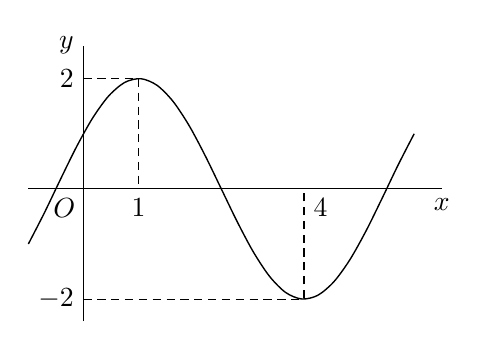
\begin{tikzpicture}[scale=0.7]
      \draw[\myaxisarrow] (-1,0) -- (6.5,0) node[below] {$x$};
      \draw[\myaxisarrow] (0,-2.4) -- (0,2.6) node[left] {$y$};
      \draw (0,0) node[anchor=45] {$O$} coordinate (O);
      \draw[line width=0.5pt,smooth,domain=-1:6] 
        plot(\x,{2*sin(\x*60+30)});

      \draw[densely dashed] (0,2) node[left] {$2$} --(1,2)--(1,0) 
        node[below] {$1$};
      \draw[densely dashed] (0,-2) node[left] {$-2$} --(4,-2)--(4,0) 
        node[below right] {$4$};
    \end{tikzpicture}
    \caption{}\label{fig-190501-1430}
    \end{minipage}
    \hskip 0.5cm%
    \begin{minipage}[b]{0.45\linewidth}
    \centering
    \begin{tikzpicture}[scale=0.7]
      \draw[\myaxisarrow] (-1,0) -- (3.5,0) node[below] {$x$};
      \draw[\myaxisarrow] (0,-2.4) -- (0,2.6) node[left] {$y$};
      \draw (0,0) node[anchor=135] {$O$} coordinate (O);
      \draw[line width=0.5pt,smooth,domain=-1:pi] 
        plot(\x,{2*sin(\x*270/pi+225)});

      \draw (-pi/6,0) node[below left] {$-\dfrac{\pi}6$};
      \draw[densely dashed] (0,2) node[left] {$2$} --(5*pi/6,2)--(5*pi/6,0) 
        node[below] {$\dfrac{5\pi}6$};
      \draw[densely dashed] (0,-2) node[left] {$-2$} --(pi/6,-2);
    \end{tikzpicture}
    \caption{}\label{fig-190501-1440}
    \end{minipage}
    \end{figure}
    
\begin{example}
    已知函数 $f(x)=2\sin(\omega x+\varphi)$ ($\omega>0$, $\pi<\varphi<\dfrac{3\pi}2$) 的部分图象如图~\ref{fig-190501-1440} 所示, 求 $f(x)$ 的表达式及其在 $\Big[\dfrac{3\pi}2, 2\pi\Big]$ 上的值域.
\end{example}
\beginsolution
    由图可知, 
    \[\left\{\!\!\begin{array}{l}
        \frac34 T= \frac{5\pi}{6}-\biggl(-\frac{\pi}{6}\biggr),\\
        f\biggl(\frac{5\pi}{6}\biggl)=2,
    \end{array}\right.\ \text{即}\ 
    \left\{\!\!\begin{array}{l}
        \frac{2\pi}\omega= \frac{4\pi}3,\\
        \sin\biggl(\frac{5\pi}{6}\omega+\varphi\biggl)= 1,
    \end{array}\right.\]
    所以 $\omega= \dfrac32$, $\sin\biggl(\dfrac{5\pi}4+ \varphi\biggr)= 1$, 解得
    \[\frac{5\pi}4+\varphi= \frac\pi2+2k\pi,\quad k\in\mathbb{Z}.\]
    由 $\pi<\varphi<\dfrac{3\pi}2$ 知 $k=1$, $\varphi= \dfrac{5\pi}4$, 即
    \[f(x)= 2\sin\biggl(\frac32 x+ \frac{5\pi}4\biggr).\]
    当 $x\in\Big[\dfrac{3\pi}2, 2\pi\Big]$ 时, $\frac32 x+ \frac{5\pi}4\in\biggl[\dfrac{7\pi}2, \dfrac{17\pi}4\biggr]$. 由三角函数的周期性, 考虑 $\frac32 x+ \frac{5\pi}4- 4\pi$ 的取值范围可知, $f(x)\in\biggl[-1,\dfrac{\sqrt2}2\biggr]$.
\endsolution

\lianxi
\begin{exercise}[s]
    若函数 $f(x)=A\sin(\omega x+\varphi)$ ($A>0$, $\omega>0$, $0<\varphi<\pi$) 的部分图象如图~\ref{fig-190501-1450} 所示, 求 $f\Big(\dfrac\pi3\Big)$ 的值.
\end{exercise}
\beginsolution
    由图可知, $A=2$ 且
    \[\left\{\!\!\begin{array}{l}
        \frac34 T= \frac{11\pi}{12}-\frac{\pi}{6},\\
        f\biggl(\frac{\pi}{6}\biggl)=2,
    \end{array}\right.\ \text{即}\ 
    \left\{\!\!\begin{array}{l}
        \frac{2\pi}\omega= \pi,\\
        2\sin\biggl(\frac{\pi}{6}\omega+\varphi\biggl)= 2,
    \end{array}\right.\]
    所以 $\omega= 2$, $\sin\biggl(\dfrac{\pi}3+ \varphi\biggr)= 1$, 解得
    \[\frac{\pi}3+\varphi= \frac\pi2+2k\pi,\quad k\in\mathbb{Z}.\]
    因为 $0<\varphi<\pi$, 所以 $k=0$, $\varphi= \dfrac{\pi}6$, 而
    \[\begin{aligned}
        f(x)&= 2\sin\biggl(2x+ \frac{\pi}6\biggr),\\
        f\biggl(\frac\pi3\biggr)&= 2\sin\biggl(2\cdot\frac\pi3+ \frac{\pi}6\biggr)
         = 2\sin\frac{5\pi}6= \sqrt3.
    \end{aligned}\]
\endsolution

    \begin{figure}[h]
    \small
    \centering
    \begin{minipage}[b]{0.45\linewidth}
    \centering
    \begin{tikzpicture}[scale=0.7]
      \draw[\myaxisarrow] (-1,0) -- (4,0) node[below] {$x$};
      \draw[\myaxisarrow] (0,-2.4) -- (0,2.6) node[left] {$y$};
      \draw (0,0) node[anchor=-45,xshift=-2pt] {$O$} coordinate (O);
      \draw[line width=0.5pt,smooth,domain=-0.6:3.2] 
        plot(\x,{2*sin(\x*360/pi+30)});

      \draw (11*pi/12,0) node[below,xshift=1em] {$\dfrac{11\pi}{12}$};
      \draw[densely dashed] (0,2) node[left] {$2$} --(pi/6,2)--(pi/6,0) 
        node[below] {$\dfrac{\pi}6$};
      \draw[densely dashed] (0,-2) node[left] {$-2$} --(2*pi/3,-2);
    \end{tikzpicture}
    \caption{}\label{fig-190501-1450}
    \end{minipage}
    \hskip 0.5cm%
    \begin{minipage}[b]{0.45\linewidth}
    \centering
    \begin{tikzpicture}[scale=1.4]
      \draw[\myaxisarrow] (-0.5,0) -- (2.5,0) node[below] {$x$};
      \draw[\myaxisarrow] (0,-1.2) -- (0,1.3) node[left] {$y$};
      \draw (0,0) node[anchor=45] {$O$} coordinate (O);
      \draw[line width=0.5pt,smooth,domain=pi/6:3*pi/4] 
        plot(\x,{sin(\x*720/pi-120)});

      \draw[densely dashed] (0,sqrt 3 /2) node[left] {$y_0$} 
        --(pi/4,sqrt 3 /2)--(pi/4,0) node[below] {$x_0$};
      \draw[densely dashed] (0,-sqrt 3/2) node[left] {$-y_0$} 
        --(pi/2,-sqrt 3 /2)--(pi/2,0)
        node[above,xshift=0.35em] {$x_0+\dfrac{\pi}4$};
    \end{tikzpicture}
    \caption{}\label{fig-190501-1500}
    \end{minipage}
    \end{figure}
    
\subsubsection{课堂评价}

\begin{exercise}
    求函数 $y=\sin2x+2\sqrt3 \sin^2 x$ 的最小正周期.
\end{exercise}
\beginsolution
    函数解析式化为
    \[\begin{aligned}
        y&= \sin2x+\sqrt3(1-\cos2x)\\
        &= \sqrt3+ 2\sin\biggl(2x- \frac\pi3\biggr),
    \end{aligned}\]
    故所求最小正周期为 $\dfrac{2\pi}2= \pi$.
\endsolution

\begin{exercise}
    求函数 $f(x)=\sin\Big(2x-\dfrac\pi4\Big)$ 在区间 $\Big[0,\dfrac\pi2\Big]$ 上的最小值.
\end{exercise}
\beginsolution
    由 $x\in\Big[0,\dfrac\pi2\Big]$ 知, $2x-\dfrac\pi4\in \Bigl[-\dfrac\pi4, \dfrac{3\pi}4\Bigr]$, 所以 $f(x)\in \biggl[-\dfrac{\sqrt2}2, 1\biggr]$.
\endsolution

\begin{exercise}
    函数 $y=\sin x$ 的图象如何变换可得到 $y=3\sin\Big(2x-\dfrac\pi3\Big)$ 的图象?
\end{exercise}
\beginsolution
    方法一: $y=\sin x$ 的图象向右平移 $\dfrac\pi3$ 得 $y= \sin\biggl(x- \dfrac\pi3\biggr)$ 的图象; 横坐标变为原来的 $\dfrac12$, 纵坐标变为原来的 $3$ 倍, 得 $y=3\sin\Big(2x-\dfrac\pi3\Big)$ 的图象.

    方法二: $y=\sin x$ 的图象横坐标变为原来的 $\dfrac12$, 纵坐标变为原来的 $3$ 倍, 得 $y=3\sin2x$ 的图象; 向右平移 $\dfrac\pi6$ 得 
    \[y= 3\sin\Bigl(2\Bigl(x- \dfrac\pi6\Bigr)\Bigr)
        = 3\sin\Bigl(2x-\dfrac\pi3\Bigr)\]
    的图象.
\endsolution

\begin{exercise}
    若函数 $y=\sin(\omega x+\varphi)$ ($\omega>0$) 
    的部分图象如图~\ref{fig-190501-1500} 所示, 求 $\omega$ 的值.
\end{exercise}
\beginsolution
    由图知, $\dfrac12 T= \dfrac\pi4$, 即
    \[\frac{2\pi}{\omega}= \frac\pi2,\quad\text{解得}\quad
        \omega= 4.\]
\endsolution
    
\subsection{课后练习}
\begin{exercise}
    求函数 $y=2\sin^2 x+3\cos^2 x-4$ 的最小正周期.
\end{exercise}
\beginsolution
    函数解析式化为
    \[\begin{aligned}
        y&= 2+\cos^2 x-4= \cos^2 x-2\\
        &= \frac{1+\cos2x}{2}- 2= \frac{\cos2x-3}{2},
    \end{aligned}\]
    故所求最小正周期为 $\dfrac{2\pi}2= \pi$.
\endsolution

\begin{exercise}
    下列哪些函数既是偶函数又在区间 $(0,\pi)$ 上单调递减?
    
    (1) $y=\sin x$;\quad (2) $y=\cos x$;\quad
    (3) $y=\sin2x$;\quad (4) $y=\cos2x$.
\end{exercise}
\beginsolution
    由各函数图象知, 仅 (2) 符合题意.
\endsolution

\begin{exercise}
    ``函数 $f(x)=\cos(2x+\varphi)$ 为奇函数'' 是 
    ``$\varphi= \dfrac\pi2$'' 的什么条件?
\end{exercise}
\beginsolution
    由 $f(x)$ 的图象知, $f(x)$ 为奇函数的充要条件是 $f(0)=0$, 即 $\cos\varphi=0$, 解得 $\varphi= \dfrac\pi2+2k\pi$, $k\in\mathbb{Z}$, 所以 ``$f(x)$ 为奇函数'' 是 ``$\varphi= \dfrac\pi2$'' 的必要不充分条件.
\endsolution

\begin{exercise}
    设 $f(x)= \sqrt3 \sin3x+\cos3x$, 若对任意的实数 $x$, 都有 $|f(x)|\leqslant a$, 求实数 $a$ 的取值范围.
\end{exercise}
\beginsolution
    函数解析式化为 $f(x)= 2\sin\Bigl(2x+\dfrac\pi6\Bigr)$, 所以 $|f(x)|\in[0,2]$, 而 $a\in[2,+\infty]$.
\endsolution

\begin{exercise}
    写出下列命题中正确的命题的序号:
    
    (1) 函数 $y=\cos\Big(\dfrac23 x+\dfrac\pi2\Big)$ 是奇函数;
    
    (2) 存在实数 $\alpha$, 使得 $\sin \alpha+\cos \alpha=2$;
    
    (3) 若 $\alpha$, $\beta$ 是第一象限角, 且 $\alpha<\beta$, 
    则 $\tan \alpha<\tan \beta$;
    
    (4) $x= \dfrac\pi8$ 是函数 $y=\sin\Big(2x+\dfrac{5\pi}4\Big)$ 的一条对称轴.
\end{exercise}
\beginsolution
    (1) $y=-\sin\dfrac23 x$ 为奇函数;

    (2) $\sin\alpha+\cos\alpha= \sqrt2\sin\Bigl(\alpha+ \dfrac\pi4\Bigr)\leqslant 2$;

    (3) 取 $\alpha= \dfrac\pi3- 2\pi$, $\beta= \dfrac\pi6$ 知 $\alpha< \beta$, 但 $\tan\alpha> \tan\beta$;

    (4) 将 $x=\dfrac\pi8$ 代入, 函数值为
    \[sin\Bigl(2\cdot \frac\pi8+ \frac{5\pi}4\Bigr)
        = \sin\frac{3\pi}2= -1,\]
    满足三角函数图象对称轴的特征.

    综上所述, (1)(4) 正确.
\endsolution

\begin{exercise}
    已知函数 $f(x)= \dfrac{(\sin x- \cos x) \sin 2x}{\sin x}$, 求其定义域、最小正周期和单调增区间.
\end{exercise}
\beginsolution
    由题意, $\sin x\neq 0$, 即定义域为 $\{x\mid x\neq k\pi,\ k\in\mathbb{Z}\}$. 函数解析式化为
    \[\begin{aligned}
        f(x)&= 2(\sin x- \cos x)\cos x\\
        &= \sin 2x-(\cos2x+1)\\
        &= \sqrt2\sin\Bigl(2x- \frac\pi4\Bigr)-1,
    \end{aligned}\]
    所以最小正周期为 $\dfrac{2\pi}2= \pi$, 单调递增区间满足
    \[2x- \frac\pi4\in \Bigl[-\frac\pi2+2k\pi, \frac\pi2+2k\pi\Bigr],\quad k\in\mathbb{Z},\]
    结合定义域知
    \[x\in \Bigl[-\frac\pi8+k\pi, k\pi\Bigr)\cup \Bigl(k\pi, \frac\pi2+k\pi\Bigr],\quad k\in\mathbb{Z}.\]
\endsolution

\begin{exercise}
    设函数 $f(x)=\sin x+\sin\Big(x+\dfrac\pi3\Big)$.
    
    (1) 求 $f(x)$ 的最小值, 并求对应的 $x$ 的集合;
    
    (2) 函数 $y=\sin x$ 的图象可由 $y=f(x)$ 的图象经过怎样的变化得到?
\end{exercise}
\beginsolution
    函数解析式化为
    \[\begin{aligned}
        f(x)&= \sin x+\frac12\sin x+ \frac{\sqrt3}{2}\cos x\\
        &= \sqrt3\biggl(\frac{\sqrt3}{2}\sin x+ \frac12\cos x\biggr)\\
        &= \sqrt3\sin\Bigl(x+\frac\pi6\Bigr).
    \end{aligned}\]

    (1) $f(x)$ 的最小值为 $-\sqrt3$, 此时
    \[x+\frac\pi6= -\frac\pi2+2k\pi,\quad k\in\mathbb{Z},\]
    所求的 $x$ 的集合为
    \[\Bigl\{x\Bigm| x= -\frac{2\pi}3+ 2k\pi,\ k\in\mathbb{Z}\Bigr\}.\]

    (2) $y= f(x)= \sqrt3\sin\Bigl(x+\frac\pi6\Bigr)$ 的图象向左平移 $\dfrac\pi6$, 得 $y= \sqrt3\sin x$ 的图象; 纵坐标变为原来的 $\dfrac1{\sqrt3}$ 倍, 得 $y= \sin x$ 的图象. 
\endsolution

\begin{exercise}
    若函数 $f(x)=A\sin(\omega x+\varphi)$ ($A>0$, $\omega>0$, $-\dfrac\pi2< \varphi< \dfrac\pi2$) 的部分图象如图 \ref{fig-190501-1520} 所示, 求 $f(x)$ 的解析式.
\end{exercise}
\beginsolution
    由图可知, $A=2$ 且
    \[\left\{\!\!\begin{array}{l}
        \frac12 T= \frac{11}{12}-\frac{5}{12},\\
        f\biggl(\frac{5}{12}\biggl)=2,
    \end{array}\right.\ \text{即}\ 
    \left\{\!\!\begin{array}{l}
        \frac{2\pi}\omega= 1,\\
        2\sin\biggl(\frac{5}{12}\omega+\varphi\biggl)= 2,
    \end{array}\right.\]
    所以 $\omega= 2\pi$, $\sin\Bigl(\dfrac{5\pi}6+ \varphi\Bigr)= 1$, 解得
    \[\dfrac{5\pi}6+ \varphi= \frac\pi2+2k\pi,\quad k\in\mathbb{Z}.\]
    因为 $-\dfrac\pi2< \varphi< \dfrac\pi2$, 所以 $k=0$, $\varphi= -\dfrac{\pi}3$, 而
    \[f(x)= 2\sin\Bigl(2\pi x- \frac{\pi}3\Bigr).\]
\endsolution

\begin{figure}[h]
    \small
    \centering
    \begin{minipage}[b]{0.45\linewidth}
    \centering
    \begin{tikzpicture}[x=2.1cm,y=0.7cm]
      \draw[\myaxisarrow] (-0.3,0) -- (1.2,0) node[below] {$x$};
      \draw[\myaxisarrow] (0,-2.4) -- (0,2.6) node[left] {$y$};
      \draw (0,0) node[anchor=45] {$O$} coordinate (O);
      \draw[line width=0.5pt,smooth,domain=0.1:1.05] 
        plot(\x,{2*sin(\x*360-60)});

      \draw[densely dashed] (0,2) node[left] {$2$} --(5/12,2)--(5/12,0) 
        node[below] {$\dfrac{5}{12}$};
      \draw[densely dashed] (0,-2) node[left] {$-2$} --(11/12,-2)
        --(11/12,0) node[above] {$\dfrac{11}{12}$};
    \end{tikzpicture}
    \caption{}\label{fig-190501-1520}
    \end{minipage}
    \hskip 0.5cm%
    \begin{minipage}[b]{0.45\linewidth}
    \centering
    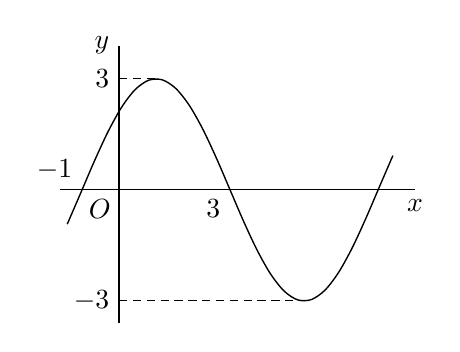
\begin{tikzpicture}[scale=0.47]
      \draw[\myaxisarrow] (-1.6,0) -- (8,0) node[below] {$x$};
      \draw[\myaxisarrow] (0,-3.6) -- (0,3.9) node[left] {$y$};
      \draw (0,0) node[anchor=45] {$O$} coordinate (O);
      \draw[line width=0.5pt,smooth,domain=-1.4:7.4] 
        plot(\x,{3*sin(\x*45+45)});

      \draw[densely dashed] (0,3) node[left] {$3$} --(1,3);
      \draw[densely dashed] (0,-3) node[left] {$-3$} --(5,-3);
      \draw (-1,0) node[above left] {$-1$} 
        (3,0) node[below left] {$3$};
    \end{tikzpicture}
    \caption{}\label{fig-190501-1530}
    \end{minipage}
    \end{figure}

\begin{exercise}
    已知 $f(x)=A\sin(\omega x+\varphi)$ ($A>0$, $\omega>0$, 
    $\varphi\in[0,\pi)$) 的部分图象如图~\ref{fig-190501-1530} 所示.
    
    (1) 求 $f(x)$ 的解析式;
    
    (2) 求函数 $g(x)=f(x)+\sqrt3 f(x+2)$ 在 $x\in[-1,3]$ 上的值域.
\end{exercise}
\beginsolution
    (1) 由图可知, $A=3$ 且
    \[\left\{\!\!\begin{array}{l}
        \frac12 T= 3-(-1),\\
        f(1)=3,
    \end{array}\right.\ \text{即}\ 
    \left\{\!\!\begin{array}{l}
        \frac{2\pi}\omega= 8,\\
        3\sin(\omega+\varphi)= 3,
    \end{array}\right.\]
    所以 $\omega= \dfrac\pi4$, $\sin\Bigl(\dfrac\pi4+ \varphi\Bigr)= 1$, 解得
    \[\dfrac\pi4+ \varphi= \frac\pi2+ 2k\pi,\quad k\in\mathbb{Z}.\]
    因为 $\varphi\in[0,\pi)$, 所以 $k=0$, $\varphi= \dfrac{\pi}4$, 而
    \[f(x)= 3\sin\Bigl(\frac\pi4 x+ \frac{\pi}4\Bigr).\]

    (2) 将 $f(x)$ 的解析式代入 $g(x)$ 的解析式,
    \[\begin{aligned}
        g(x)&= 3\sin\Bigl(\frac\pi4 x+ \frac\pi4\Bigr)
            + \sqrt3\cos\Bigl(\frac\pi4 x+ \frac\pi4\Bigr)\\
        &= 2\sqrt3\sin\Bigl(\frac\pi4 x+ \frac\pi4+ \frac\pi6\Bigr)\\
        &= 2\sqrt3\sin\Bigl(\frac\pi4 x+ \frac{5\pi}{12}\Bigr).
    \end{aligned}\]
    因为 $x\in[-1,3]$, 所以
    \[\frac\pi4 x+ \frac{5\pi}{12}\in \Bigl[\frac\pi6, \frac{7\pi}{6}\Bigr],\]
    而 $g(x)\in[-\sqrt3, 2\sqrt3]$.
\endsolution

%%%%%%%%%%%%%%%%%%%%%%%%%%%%%%%%